\documentclass[report.tex]{subfiles}
\begin{document}
\subsection{Results}
A sample output of the schematic simulation of a Microstrip Coupled-line filter is shown in \ref{fig:filter simulation sample}.

In table~\ref{table:attenuation summary}, the various pass- and stop-band limit attenuations are listed.

Figure~\ref{fig:S-parameters lab3} show the schematic simulation of the lumped component band-pass filter and the layout simulation of the various distributed band-pass filters.

\clearpage

% Let's fill some space
\vspace*{\fill}

\begin{figure}[h]
    \centering
    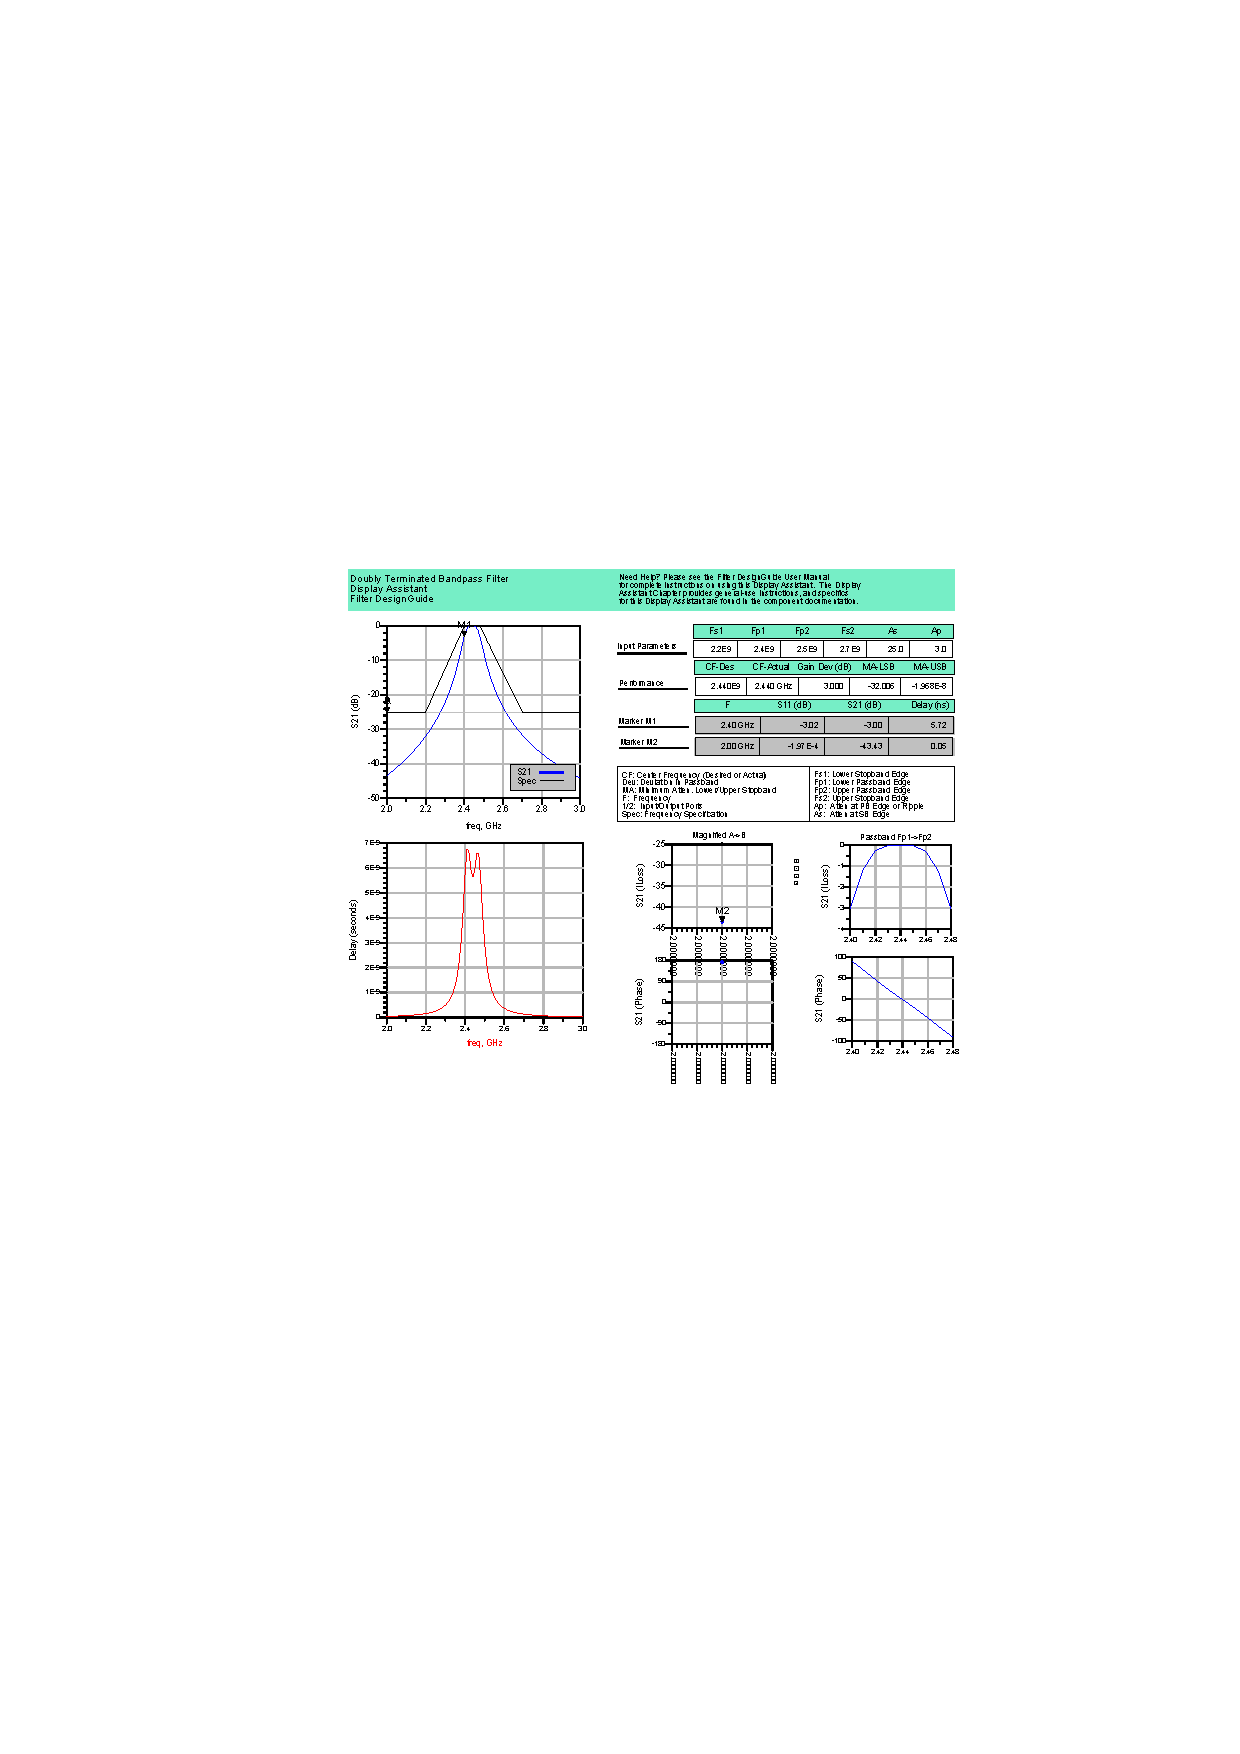
\includegraphics[width=0.7\linewidth]{filter_simulation_example}
    \caption{Schematic simulation of a Microstrip Coupled-line filter}
    \label{fig:filter simulation sample}
\end{figure}

% Let's fill some space
\vspace*{\fill}

\begin{table}[h]
    \centering
    \caption{Attenuations at pass- and stop-band limits}
    \begin{tabular}{l | c | c | c | c }
    \multicolumn{1}{c}{} & \multicolumn{4}{c}{Attenuation [-dB]\footnotemark[1]} \\
    & f=2.2 GHz & f=2.4 GHz & f=2.48 GHz & f=2.7 GHz \\
    \hline
    Lumped components                & 32.0/-    & 3.0/-   & 3.0/-   & 31.7/-    \\
    Distributed 2\nd order (RO4350B) & 14.8/16.6 & 3.6/6.2 & 3.9/2.2 & 12.7/12.6 \\
    Distributed 2\nd order (FR-4)    & -/21.6    & -/17.0  & -/14.7  & -/2.8     \\
    Distributed 3\rd order (FR-4)    & -/43.5    & -/35.0  & -/30.6  & -/3.0     \\
    \end{tabular}
    \label{table:attenuation summary}
\end{table}
\footnotetext[1]{Schematic simulation/layout simulation}
\pagebreak
%\begin{figure}[h]
%    \centering
%    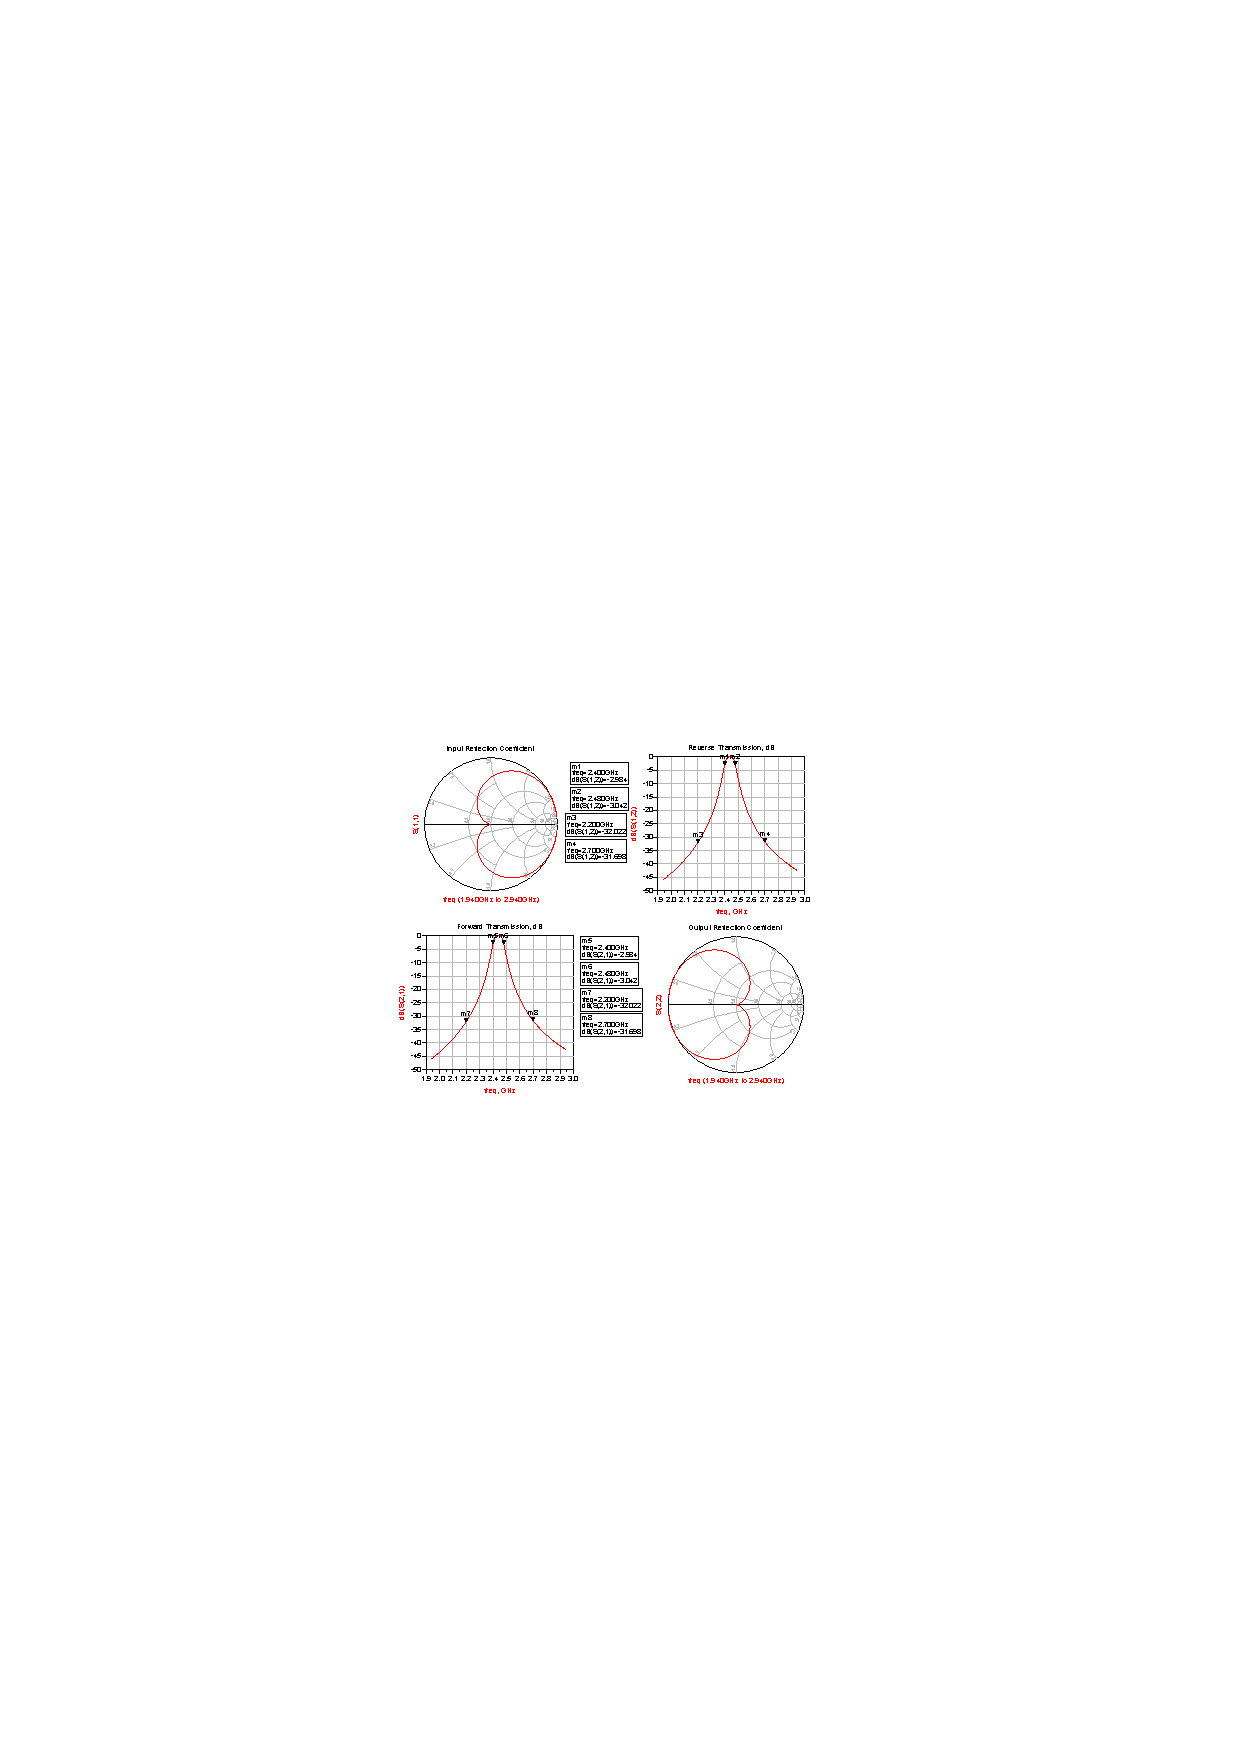
\includegraphics[width=0.8\linewidth]{S-params_filter_A}
%    \caption{S-parameters vs. frequency of lumped 2\nd order band-pass filter}
%\end{figure}

%\begin{figure}[h]
%    \centering
%    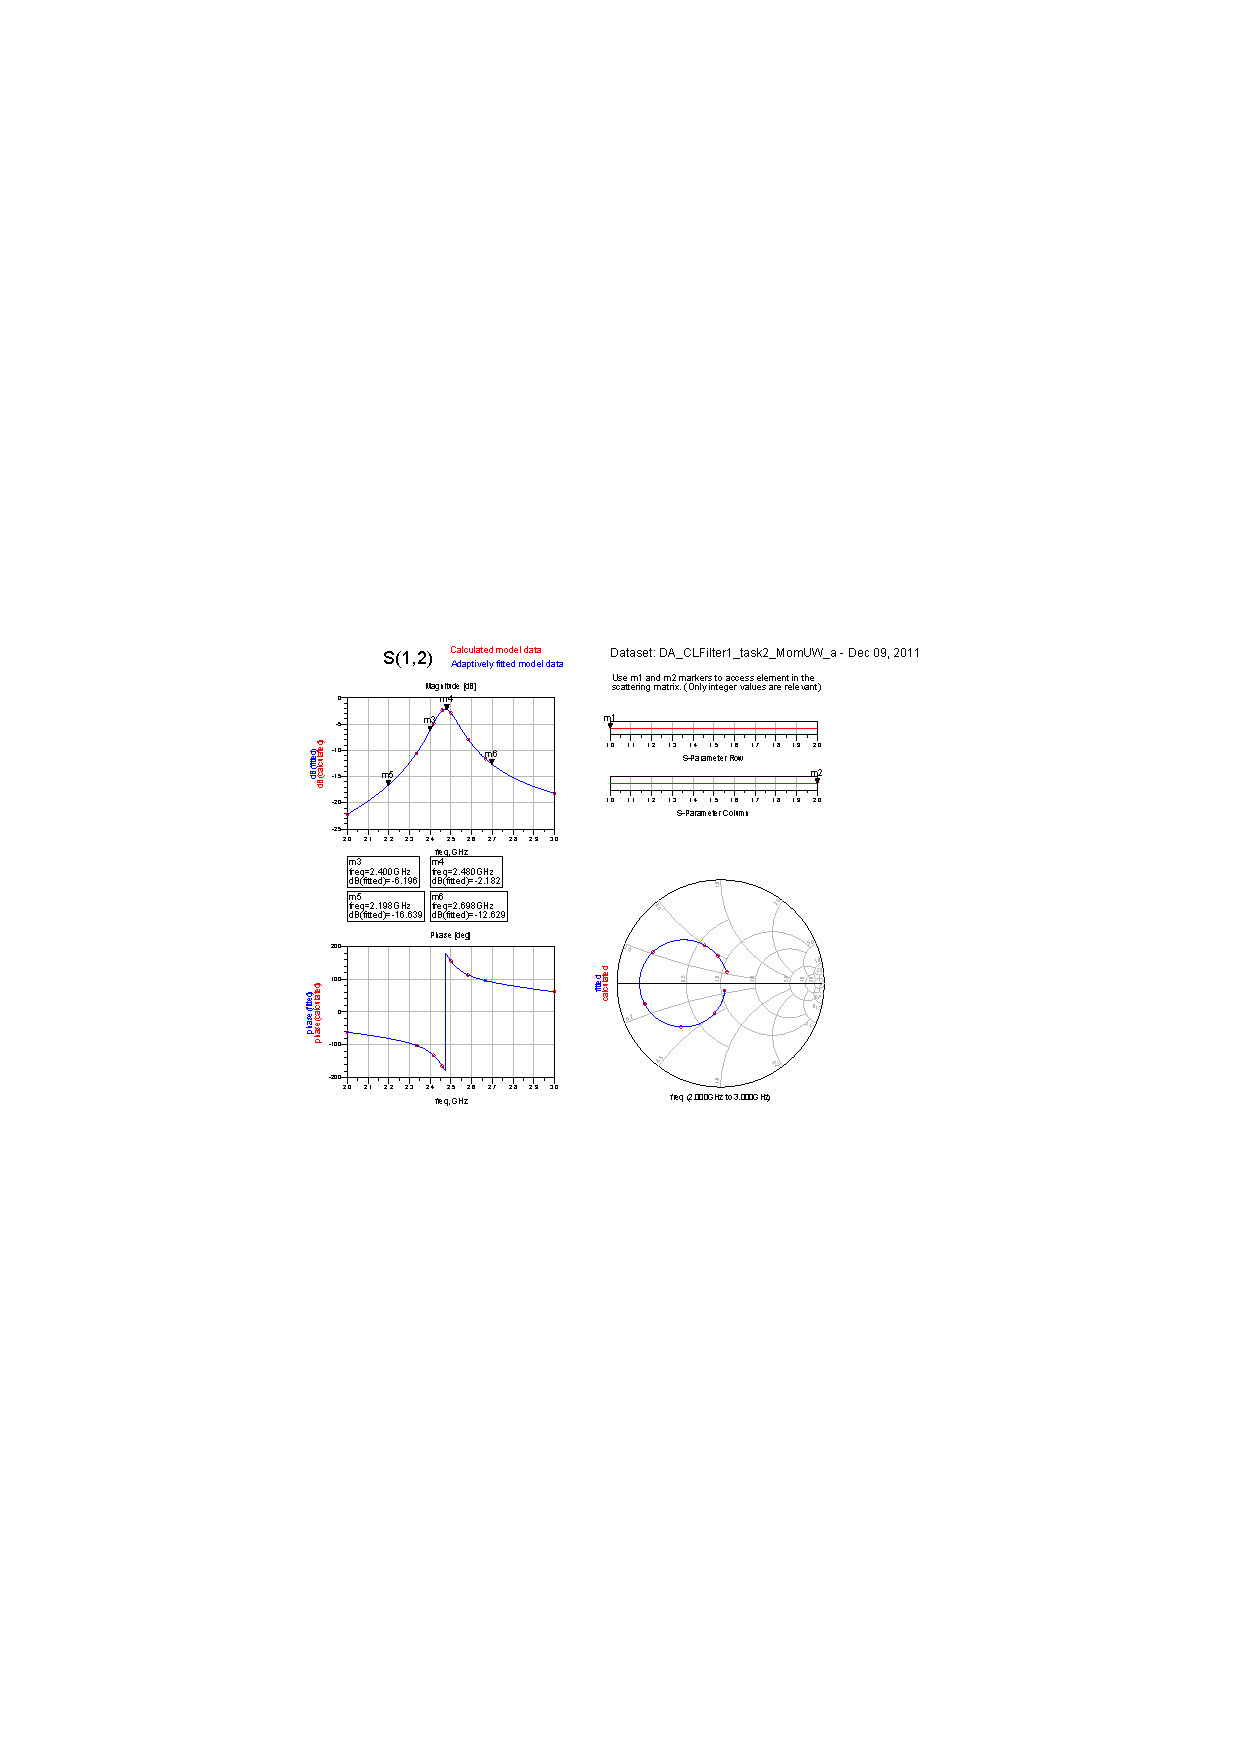
\includegraphics[width=0.8\linewidth]{S-params_filter_B}
%    \caption{S-parameters of distributed 2\nd order band-pass filter (RO4350B)}
%\end{figure}

%\begin{figure}[h]
%    \centering
%    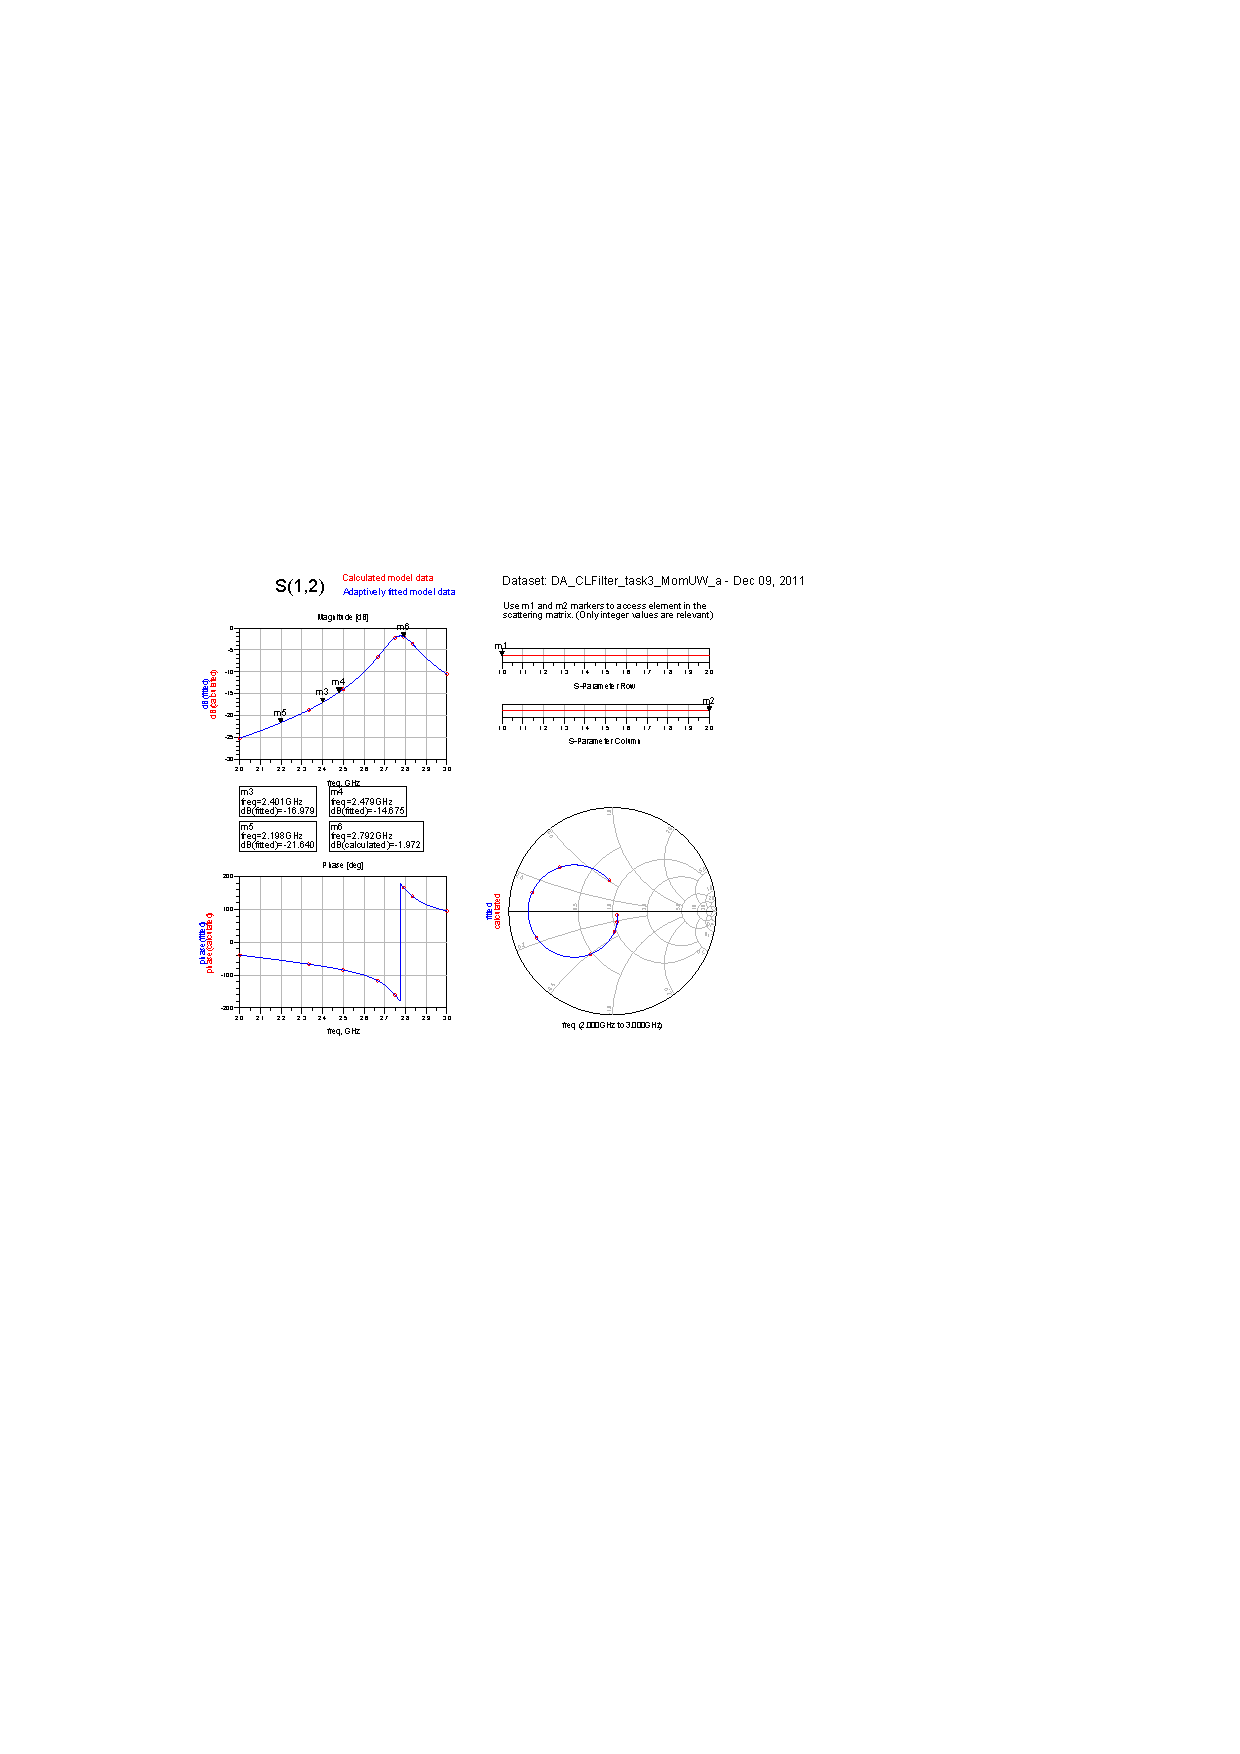
\includegraphics[width=0.8\linewidth]{S-params_filter_C}
%    \caption{S-parameters of distributed 2\nd order band-pass filter (FR-4)}
%\end{figure}

%\begin{figure}[h]
%    \centering
%    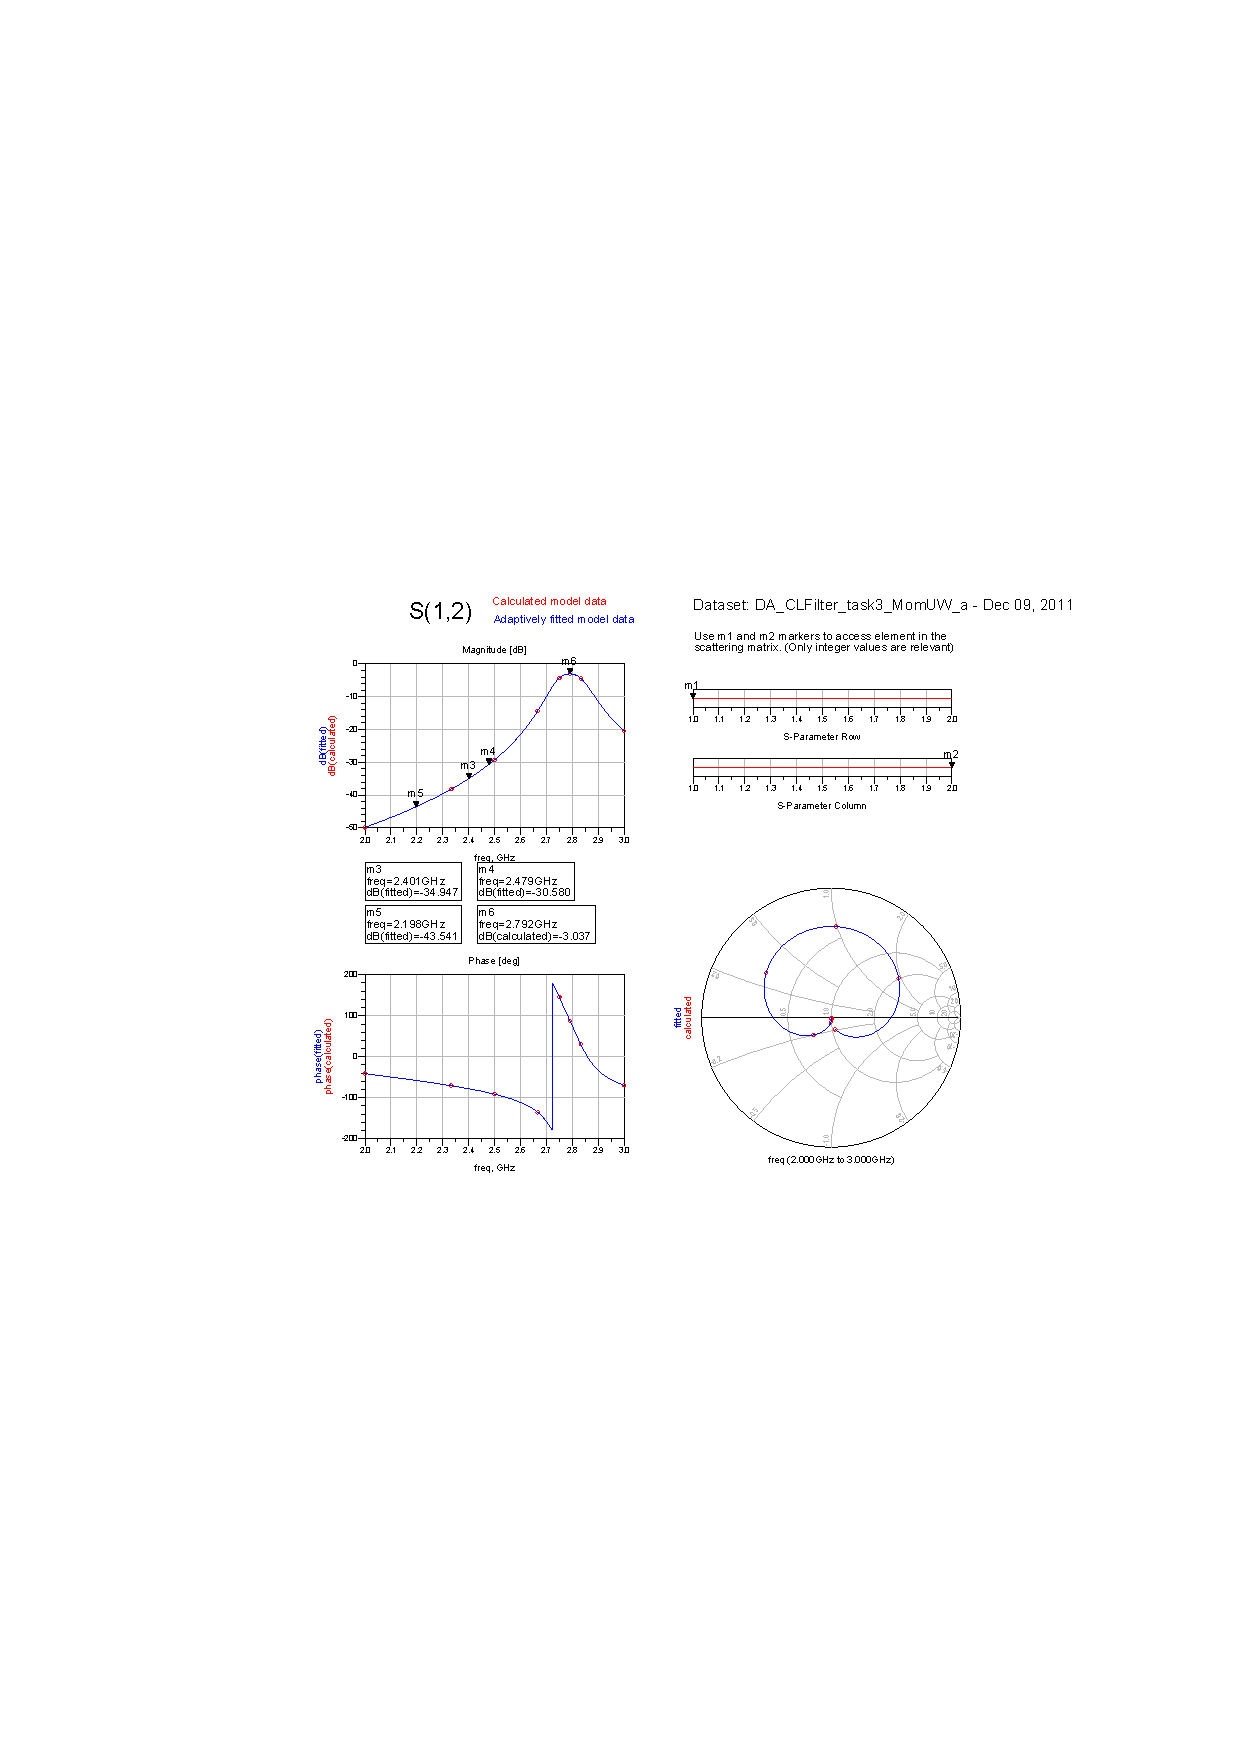
\includegraphics[width=0.8\linewidth]{S-params_filter_C_auto-N}
%    \caption{S-parameters of distributed 3\rd order band-pass filter (FR-4)}
%\end{figure}
%\clearpage

\begin{figure}
    \centering
    \vspace*{\fill}
    \subfloat[Lumped components, 2\nd order]{
        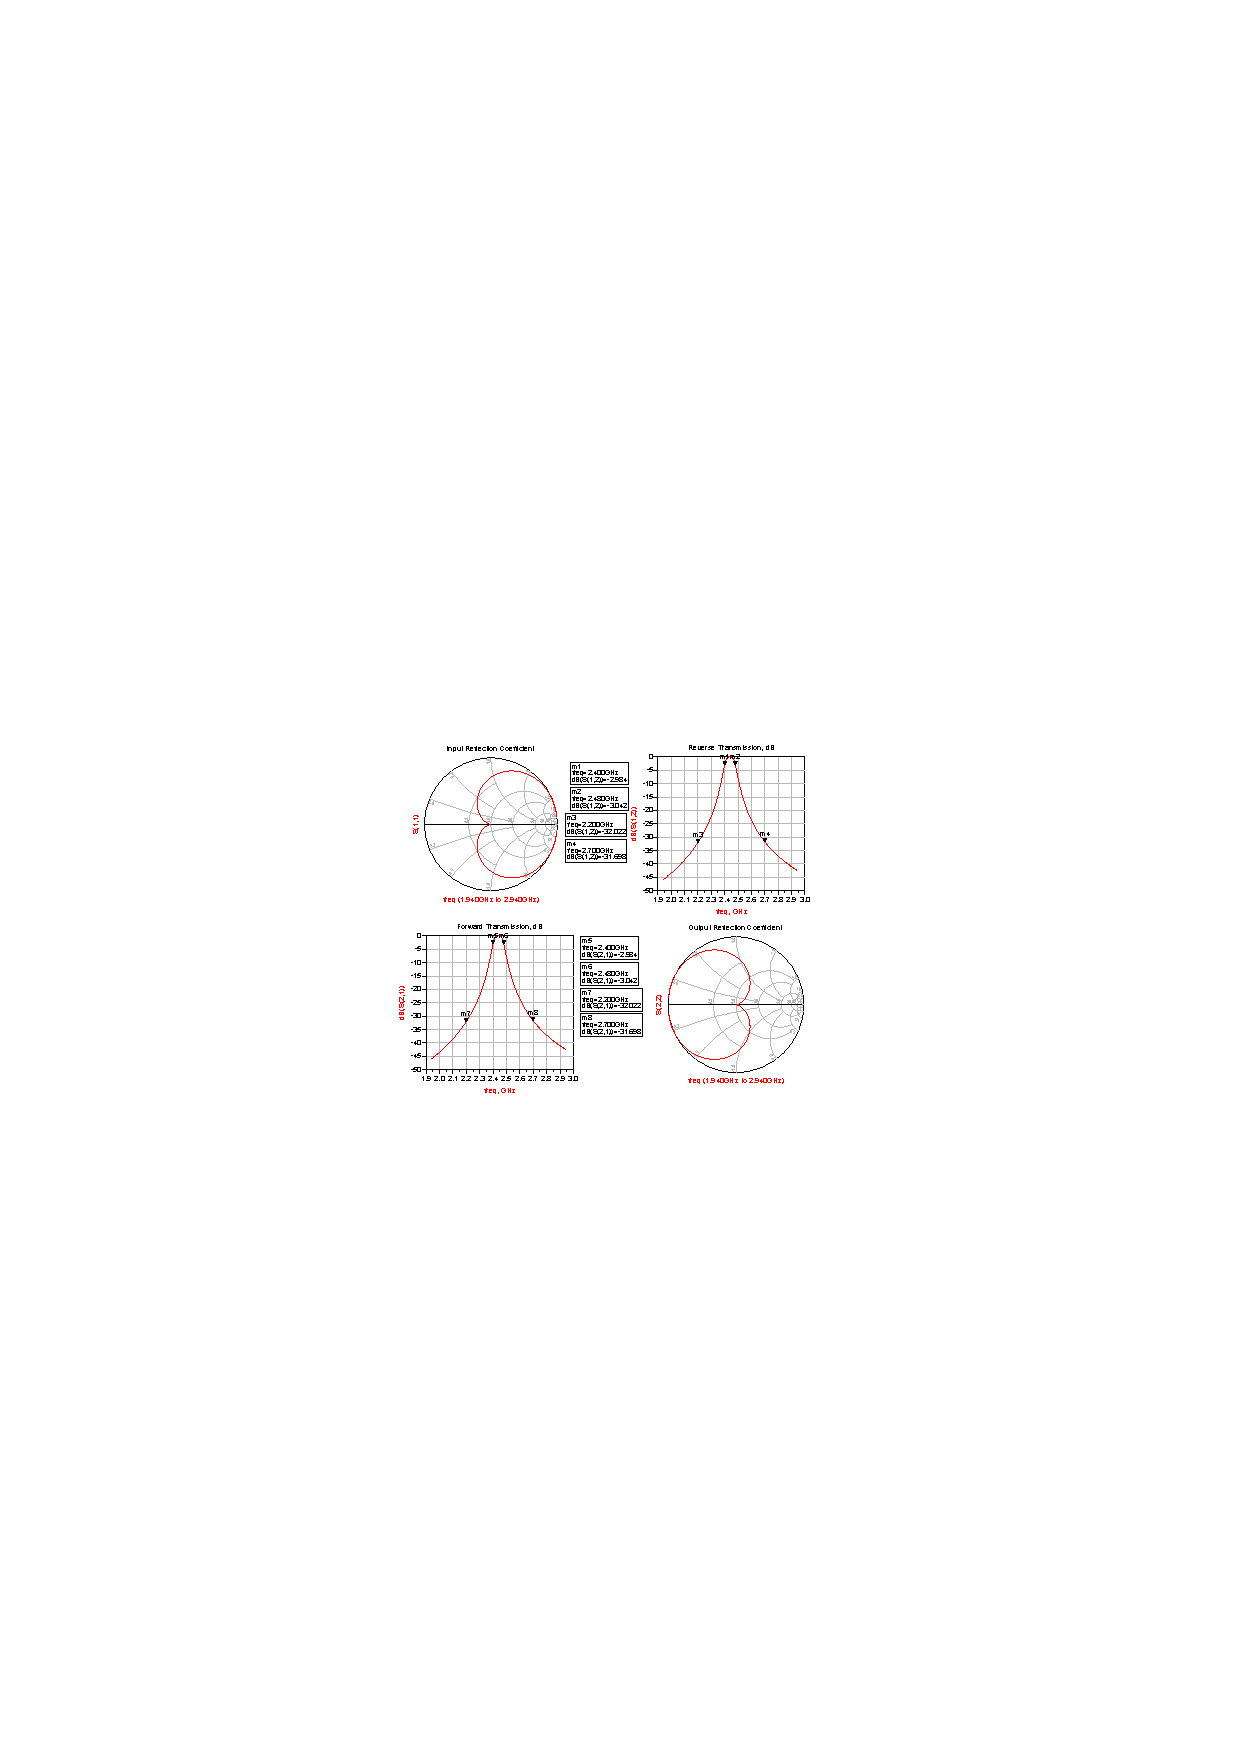
\includegraphics[width=0.5\linewidth]{S-params_filter_A}
    }
    \subfloat[Distributed (RO4350B), 2\nd order]{
        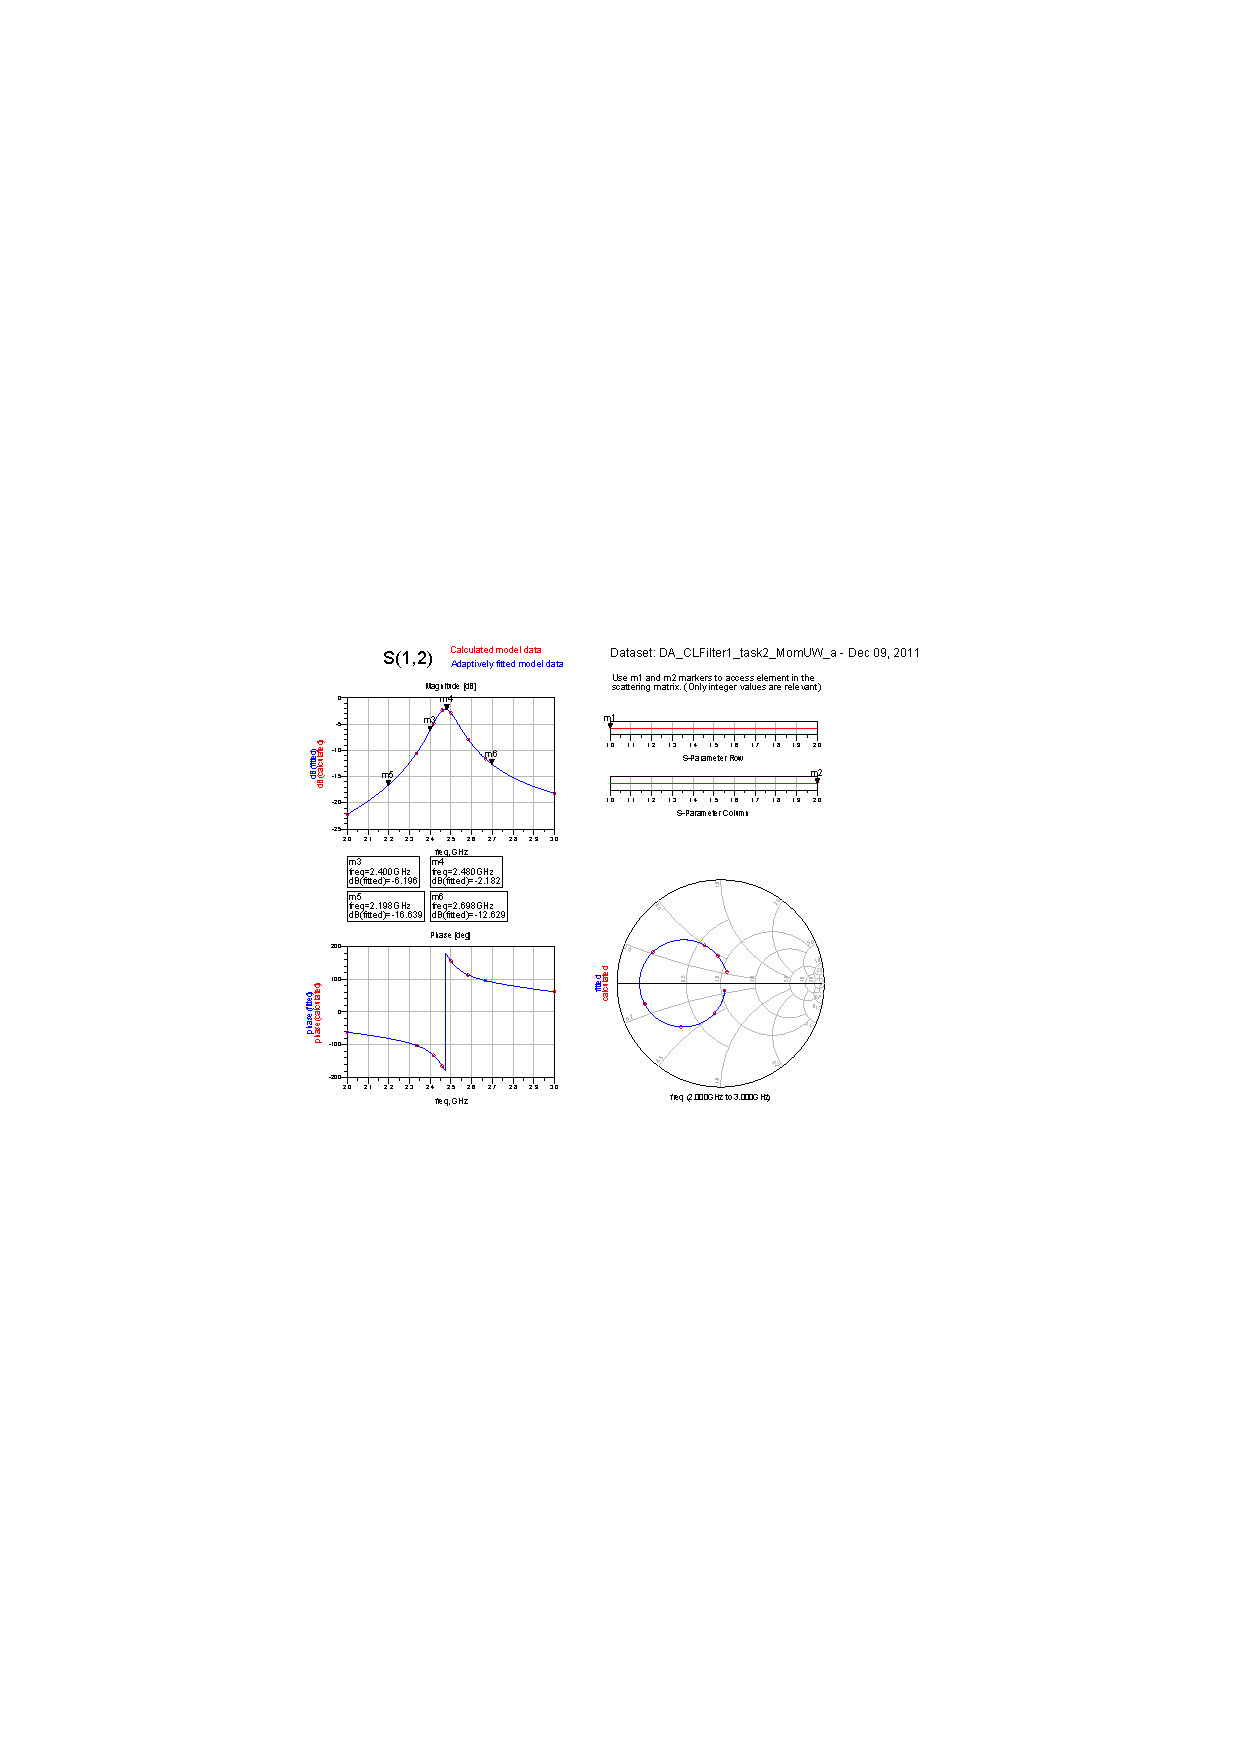
\includegraphics[width=0.5\linewidth]{S-params_filter_B}
    }
    
    \subfloat[Distributed (FR-4), 2\nd order]{
        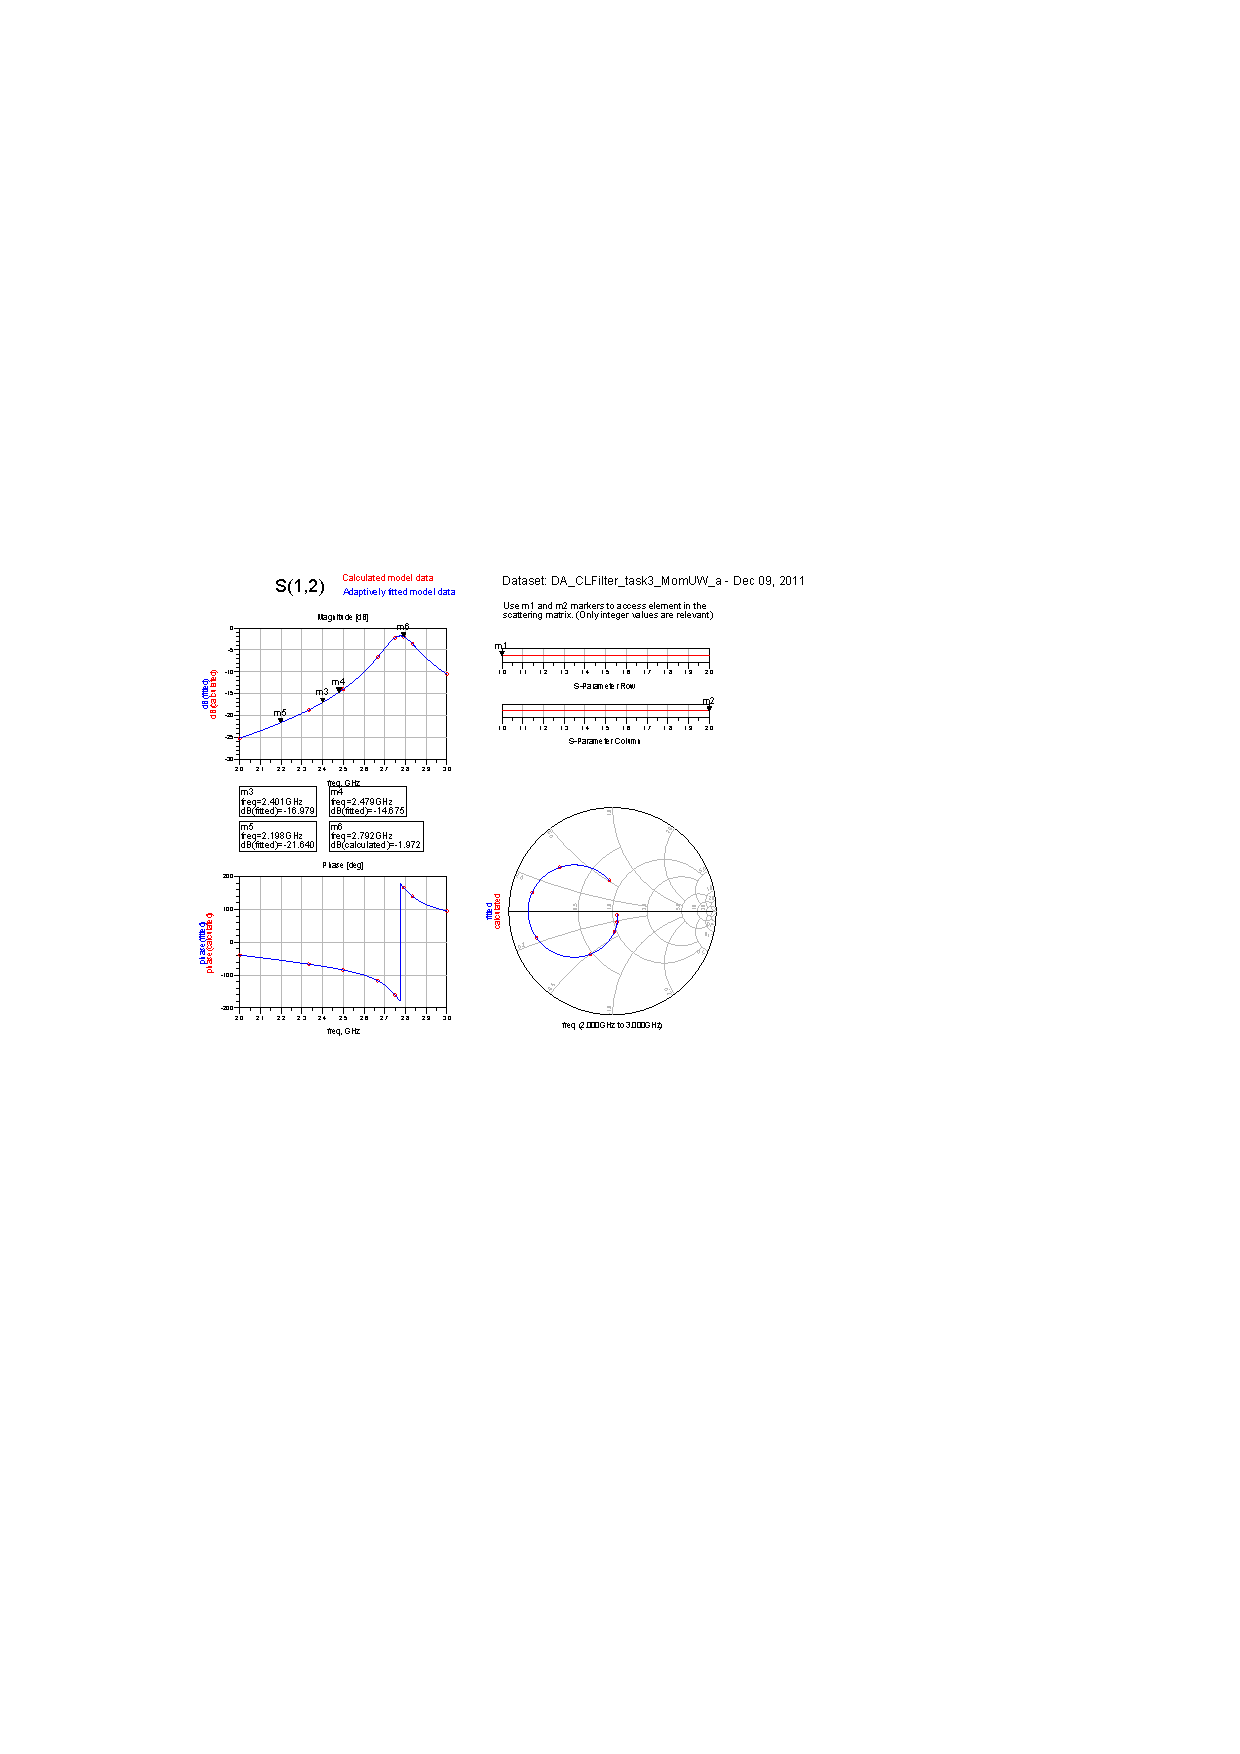
\includegraphics[width=0.5\linewidth]{S-params_filter_C}
    }
    \subfloat[Distributed (FR-4), 2\rd order]{
        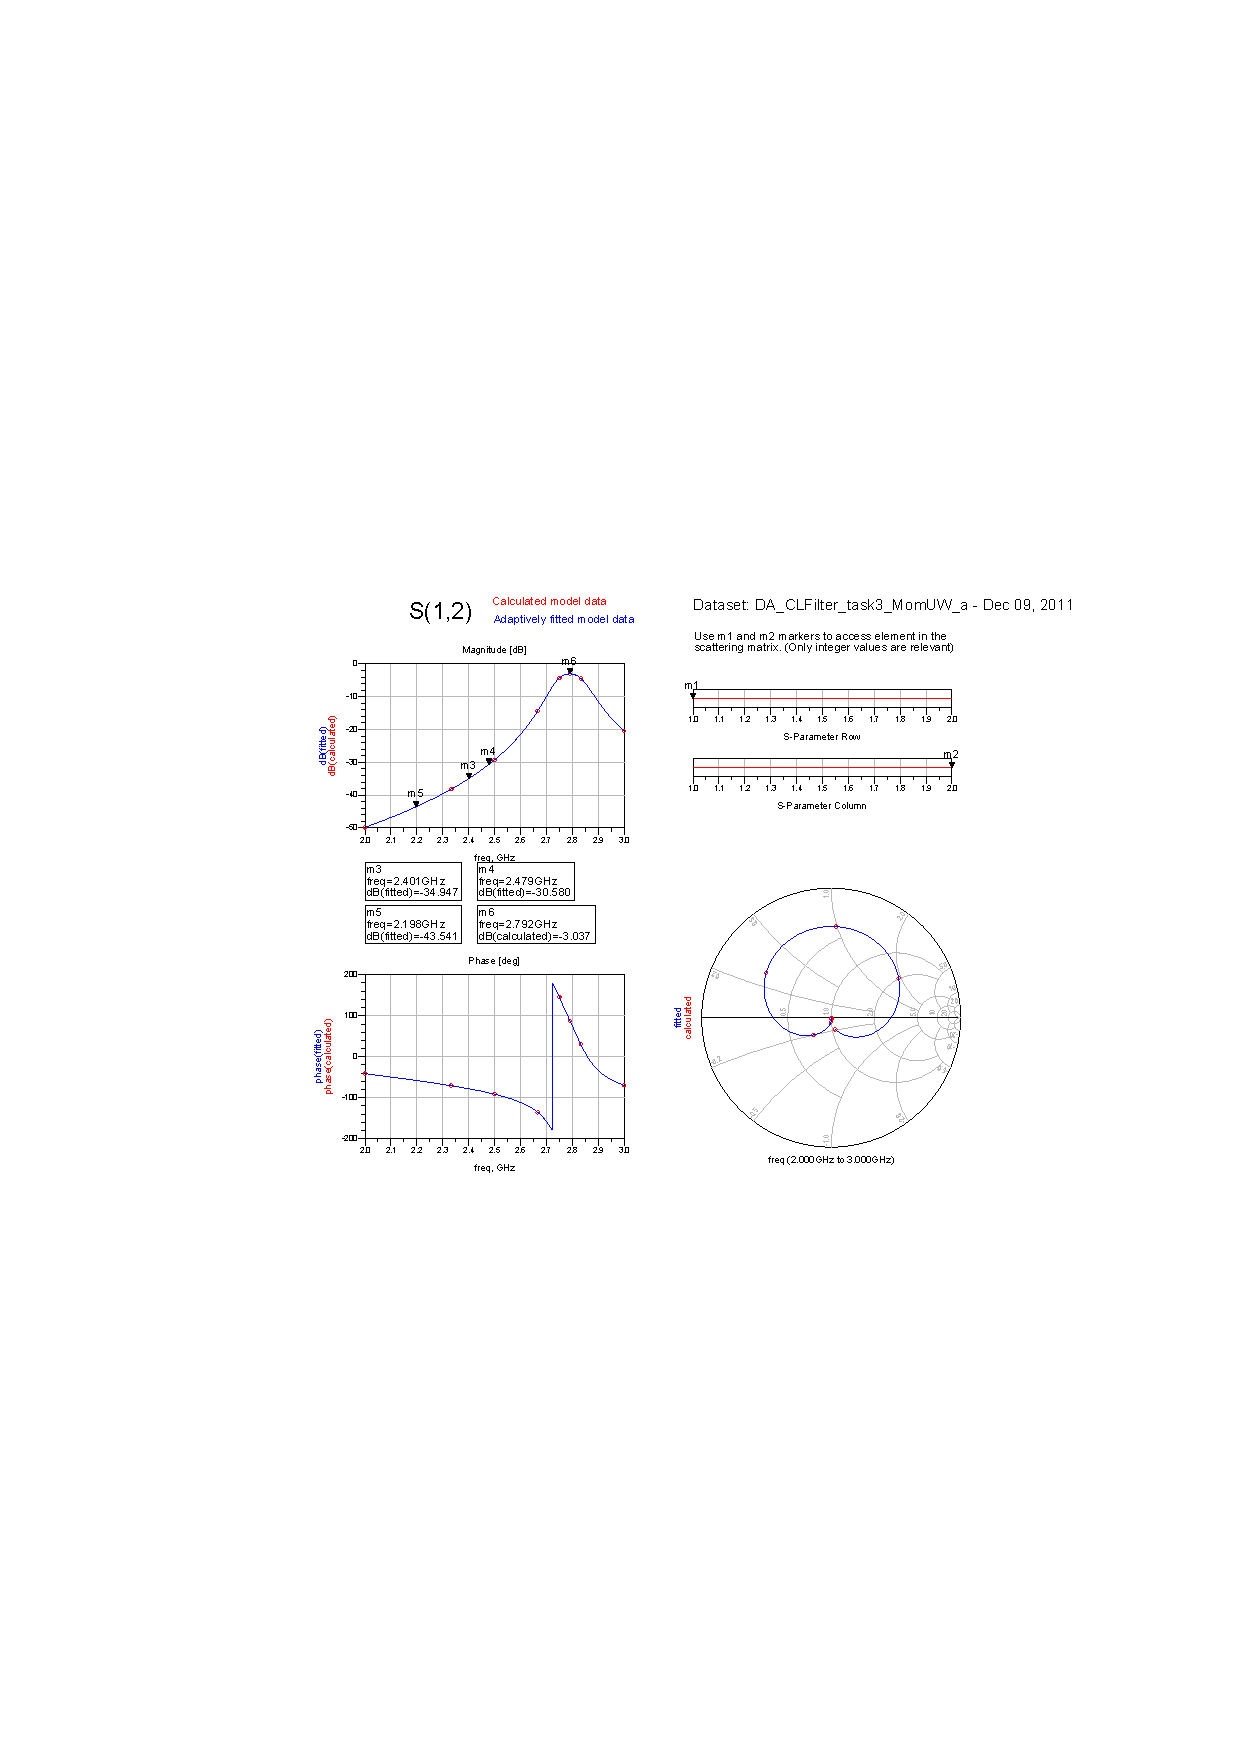
\includegraphics[width=0.5\linewidth]{S-params_filter_C_auto-N}
    }
    \caption{S-parameters vs. frequency of maximally flat band-pass filters}
    \label{fig:S-parameters lab3}
    \vspace*{\fill}
\end{figure}
\clearpage

\end{document}